\chapter{The \fshark{} Wrapper}
In this chapter we will first demonstrate how to compile and use an \fshark{}
module within an \fsharp{} project.
Then, we will explain the \fshark{} Compiler and it's pipeline.

mere here

Although \fshark{} code can be executed directly in \fsharp{} as normal
\fsharp{} code, our benchmarks in chapter \ref{chap:evaluation} shows
that compiling our \fshark{} code to Futhark OpenCL modules gives us performance
increases by several orders of magnitudes (from $\times 100~\text{to}~\times 1000$).

\section{Using the \fshark{} Wrapper}
\label{sec:fsharkcompiler}

\subsection{Another short \fshark{} module}
\begin{figure}[H]
  \centering
\begin{minted}[linenos]{fsharp}
module ExampleModule
open FSharkPrelude

let saxpy (a : int) (x : int) (y : int) : int =
  a*x+y

let getArrayPair (a : int) : (int array * int array) =
  let xs = Iota a
  let n = Length xs
  let ys = Rotate (n / 2) xs
  in (xs, ys)

[<FSharkEntry>]
let entry (a : int) : int array =
  let (xs, ys) = getArrayPair a
  let res = Map2 (saxpy a) xs ys
  in res
\end{minted}
  \caption{A short \fshark{} module in a file named ExampleModule.fs}
  \label{fig:fsharkusageexample0}
\end{figure}

In figure \ref{fig:fsharkusageexample0} we see a simple \fshark{} module that we
want to compile into a GPU kernel and use in our \fsharp{} program.
\\
Line by line, this module does the following:\\
\textbf{L1:} We define the name of this module as \texttt{ExampleModule}. If we
want to use this module in an \fsharp{} program without compiling it as
\fshark{} first, we can refer to this module by this name.
\\
\textbf{L2:} We open \fshark{}s standard library \texttt{FSharkPrelude} in this
module, so we can access the standard functions in the \fshark{} module.
In this module, we are using the standard functions \texttt{Iota}, \texttt{Length}, \texttt{Rotate} and \texttt{Map2}.
\\
\textbf{L4-5:} We define the function \texttt{saxpy}.
\\
\textbf{L7-11:} We define the function \texttt{getArrayPair}.
\\
\textbf{L8:} \texttt{Iota a} returns the integer array of the numbers from $0$
up to, but not including, $a$.
\\
\textbf{L9:} \texttt{Length xs} returns the length of the array \texttt{xs}.
\\
\textbf{L10:} \texttt{Rotate n} rotates the contents of an array n places in
either the right or left direction.\\
In example, \texttt{Rotate 2 [1;2;3;4;5;6] = [5;6;1;2;3;4]},\\
and \texttt{Rotate (-2) [1;2;3;4;5;6] = [3;4;5;6;1;2]}
\\
\textbf{L11:} Here we return the pair of arrays \texttt{(xs, ys)}.

\textbf{L13-17:} We define the entry function \texttt{entry}.\\
\textbf{L15:} We call \texttt{getArrayPair} to get two arrays.\\
\textbf{L16:} We use \texttt{Map2} to map the curried function \texttt{(saxpy
  a)}
over the arrays \texttt{xs} and \texttt{ys}.

For two arrays $\mathtt{xs} =
[\mathtt{x}_1,~\mathtt{x}_2,~\ldots,~\mathtt{x}_n]$ and $\mathtt{ys} =
[\mathtt{y}_1,~\mathtt{y}_2,~\ldots,~\mathtt{y}_n]$,\\
$\mathtt{Map2}~\mathtt{(saxpy~a)}~\mathtt{xs}~\mathtt{ys}} = [\mathtt{saxpy~a}~\mathtt{x}_1~\mathtt{y}_1, \mathtt{saxpy~a}~\mathtt{x}_2~\mathtt{y}_2,\ldots,~\mathtt{saxpy~a}~\mathtt{x}_n~\mathtt{y}_n]$.
\textbf{L17:} The entry function returns the result of the call to \texttt{Map2}.

This concludes the short \fshark{} module.
\clearpage

\subsection{Compiling and using the short \fshark{} module}
\label{compilingandusingfsharkmodule}
With our \fshark{} module ready, we now proceed to compile, load and use it.
\begin{figure}[h]
  \centering
    \begin{minted}[linenos,breaklines]{fsharp}
module FSharkExample
open FShark.Main

[<EntryPoint>]
let main argv =
  let wrapper = 
    new FSharkWrapper(
      libName="ExampleModule",
      tmpRoot="/home/mikkel/FShark",
      preludePath= "/home/mikkel/Documents/fshark/FSharkPrelude/bin/Debug/FSharkPrelude.dll",
      openCL=true,
      unsafe=true,
      debug=false
      )
  wrapper.AddSourceFile "ExampleModule.fs"
  wrapper.CompileAndLoad
  let a = 1000000
  let result = wrapper.InvokeFunction("entry", a) :?> int array
  printfn "Mapping (+2) over %A gives us %A" xs xs'
  0
    \end{minted}
  \caption{An F\# program using \fshark{}}
  \label{fig:fsharkusageexample}
\end{figure}

\textbf{L6:} We begin by constructing an instance of the \fshark{}Wrapper. It has the following
mandatory arguments:

\begin{description}
\item[\texttt{libName}]\hfill\\
  This is the library name for the \fshark{} program. In the final Futhark
  \texttt{.cs} and \texttt{.dll} files, the main class will have the same name
  as the \texttt{libName}. This doesn't really matter if \fshark{} is just used
  as a JIT compiler, but it's good to have a proper name if the user only wants
  to use the compiler parts of \fshark{}.

\item[\texttt{tmpRoot}]\hfill\\
  The \fshark{} compiler works in its own temporary directory. This argument must
  point to a directory where F\# can write files and execute subprocesses
  (Futhark- and C\# compilers) which also has to write files.
  
\item[\texttt{preludePath}]\hfill\\
  The \fshark{} compiler needs the FShark prelude available to compile FShark
  programs. 

\item[\texttt{openCL}]\hfill\\
  Although Futhark (and therefore \fshark{}) is most effective on OpenCL-enabled
  computers, the benchmarks in \ref{sec:benchmarks} still show a significant
  speed increase for non-OpenCL Futhark over native F\# code.
  Therefore, \fshark{} is also available for non-OpenCL users. Use this flag to
  tell \fshark{} whether Futhark should compile C\# with or without OpenCL.
  
\item[\texttt{unsafe}]\hfill\\
  For some Futhark programs, the Futhark compiler itself is unable to tell
  whether certain array operations or SOAC usages are safe, and will stop the
  compilation, even though the code should (and does) indeed work.
  To enable these unsafe operations, pass a \texttt{true} flag to the compiler.

\item[\texttt{debug}]\hfill\\
  Passing the debug flag to the \fshark{} compiler enables various runtime
  debugging features, for instance benchmarking the time it takes to run various
  parts of the compiler.
\end{description}

\textbf{L15:} Now we can pass a source file to the \fshark{} wrapper. \\
\textbf{L16:} We tell the wrapper to compile the source file that we have added
to the wrapper object, and load the compiled library into the wrapper
afterwards.
\textbf{L17:} As our entry function defined in the module in figure
\ref{fig:fsharkusageexample0} takes an integer as argument, we define an integer
variable we can pass to it.
\textbf{L18:} We use the wrapper to invoke the entry function from the compiled
and loaded library, using our previously declared \texttt{a} as the only
argument. As the \fshark{} wrapper uses reflection to dynamically load compiled
libraries at runtime, we are not able to statically determine what type of
result we will get from the \texttt{InvokeFunction} call. Therefore, we use F\#s
downcast operator \texttt{(:?>)} to declare the return value as an \texttt{int
  array}.

If we are in doubt of which type to downcast to, we can always lookup the return
type by reviewing the \fshark{} module's source code. We can downcast to any of
the types usable in \fsharp{}, including tuples and arrays.

\section{On the design decisions of the \fshark{} wrapper}
To summary the current design of \fshark{} usage, \fshark{} is dependent on a
wrapper object, which for all \fshark{} projects must compile the load the input
\fshark{} modules once, and afterwards passes arguments from \fsharp{} to the
resulting GPU kernels by using .NET reflection.
This design has several costs for both usability and performance, and we will
here discuss some of these costs, and what we could do to alleviate them in the
future.

\subsection{Compiling and loading \fshark{} modules at every startup}
At this time, \fshark{} works by compiling and loading \fshark{} modules just in
time before they are needed in the containing \fsharp{} project. However, this
is more often than not redundant work. For the developer who is using \fshark{} to develop
prototypes of \fshark{} GPU kernels, it is of course beneficial to continuously
recompile the \fshark{} program under development to verify the changes being
made.

However, when the \fshark{} program is finished and ready to be used in
projects, it isn't necessary to compile it again.

\subsubsection{How much time do we spend on compiling and loading the \fshark{} modules?}
If we, instead of loading the compiled \fshark{} GPU kernels through the
\fshark{} wrapper, just open the compiled kernel libraries as any other
\csharp{} \texttt{.dll} file, we can circumvent the \fshark{} compiler
completely, and use the compiled kernel directly.

For the two benchmarks \texttt{LocVolCalib} and \texttt{nbody}(see sec
\ref{benchmarks}), we have compared the time cost of the two different
approaches. In figure \ref{benchmarkcalculations} we see how the time is spent
in the two different methods.
\begin{figure}[H]
  \centering
  \begin{tabular}{@{}l c r c l c r}
 Parsing \fshark{} code using \fsharp{} parser          & &   217984 ms & $\vrule$ & & & \\
    Converting \fsharp{} declarations to FSharkIL       & &+   19129 ms & $\vrule$ & & & \\
 Converting FSharkIL to Futhark source code             & &+   98949 ms & $\vrule$ & & & \\
 Compiling Futhark to \csharp{} with \texttt{futhark-cs}& &+ 8037165 ms & $\vrule$ & & & \\
 Compiling \csharp{} code using \csharp{} compiler      & &+  999251 ms & $\vrule$ & & & \\
 Loading compiled \csharp{} class using reflection      & &+  101601 ms & $\vrule$ & Loading and constructing class from library & &  \\
  \end{tabular}
  \caption{Time spent on making LocVolCalib available in \fshark{}-using
    program}
  \label{benchmarkcalculations}
\end{figure}

MORE BENCHMARKS

WE ARE OBVIOUSLY WASTING TIME

\subsubsection{Suggestions for changes}
We have two main suggestions for change.\\
1) The easiest way would be to add a \texttt{AddModulePath} function to the
\fshark{} wrapper. The benchmarks show that we aren't spending that much more
time when loading compiled assemblies into \fsharp{} using reflection, than if
we opened the assembly as a library in the project.

Therefore, we could add a function that takes a path to a compiled \fshark{}
module, and loaded the path's target into the wrapper.

2) We could also go for a second, more permanent solution. Instead of relying on
\fsharp{}s reflection functionality to load our compiled assemblies into scope
dynamically, we could redesign the \fshark{} use case itself, so that it uses
just the compiler, and not the wrapper.

In this case, the new use case would be to compile the \fshark{} modules using
the \fshark{} compiler, and then manually reference- and open them in \fsharp{} projects.
This would not only remove the repeated module compilation, but also let us use
static typing with the compiled \fshark{} modules, enabling autocompletion and
type checking for function arguments, and also removing the need to manually
downcast the \fshark{} invokation results.

\subsection{The overhead of invoking GPU kernels}
The second issue with the current approach is, that every single call to a
\fshark{} function carries significant overhead for copying data back and forth
between CPU and GPU buffers.
This is a problem when we are chaining together GPU function calls: that is when
we take the array output of function $f$ and use it as an argument for function
$g$ without any changes to it.

In figure \ref{fig:witharraycopying} we see a chain of three calls to a compiled \fshark{} module. 
Although we are calling the second function with the result from the first
function together with another array, and calling the third function with result
from the second function, we are still moving the results from the GPU buffers to our system RAM between each call, and deallocating
the buffers on the GPU, even though we are going to reallocate them soon
thereafter.

\begin{figure}[H]
  \centering
  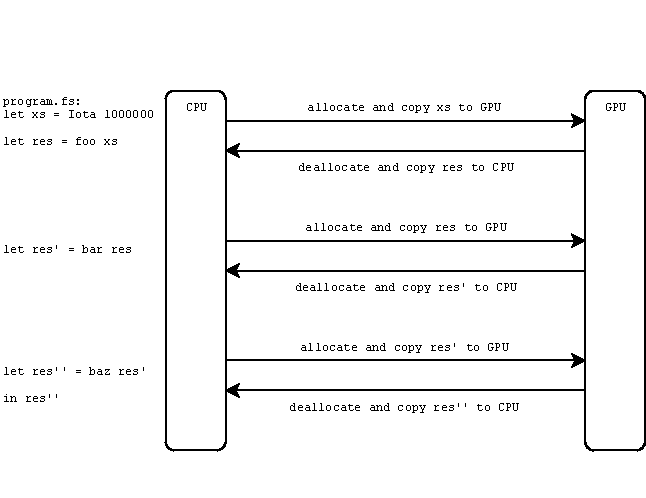
\includegraphics[scale=1.15]{chapters/figs/witharraycopying.pdf}
  \caption{Buffers are copied back and forth between CPU and GPU between calls}
  \label{fig:witharraycopying}
\end{figure}


In the future, we could eliminate this overhead by allowing the compiled Futhark functions
to return references to GPU buffers instead of indiscriminately returning
actual data arrays.
We could then also have multiple versions of the compiled Futhark functions; one
version that takes an actual data array as input, and one that can use a
reference to a GPU buffer instead.

In this case, we could wait until after the three function calls to actually
copy the referenced GPU buffer back to the system RAM. This would strongly reduce the
number of copies back and forth between the GPU and the system RAM:
Instead of the allocations/deallocations increasing linearly with the number of
chained GPU kernel calls, we can make do with one allocation and one
deallocation between system RAM and GPU, pr. chain, as in figure \ref{fig:withoutarraycopying}
\begin{figure}[H]
  \centering
  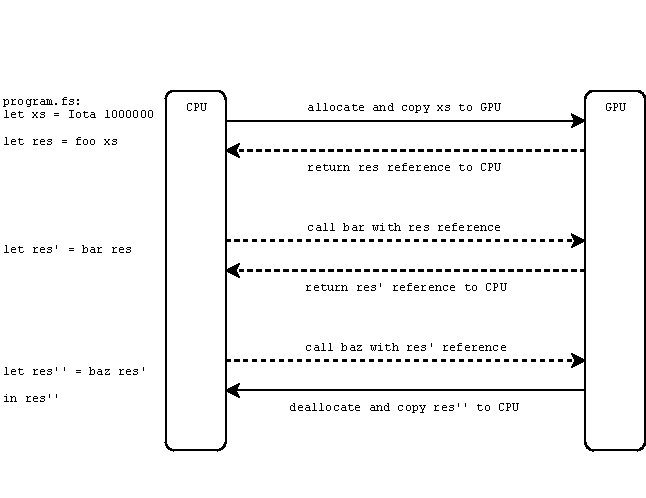
\includegraphics[scale=1.15]{chapters/figs/withoutarraycopying.pdf}
  \caption{Buffers aren't copied between CPU and GPU unless necessary}
  \label{fig:withoutarraycopying}
\end{figure}

This functionality is already implemented in Python's \texttt{PyOpenCL} library,
and is used in Futhark programs that are compiled as Python libraries.
\clearpage

\chapter{The \fshark{} Compiler}

Parsing and building a regular F\# program is trivial when using official build tools like
\texttt{msbuild} or \texttt{fsharpc}.
But in the case of \fshark{}, we are not interested in the final result from the
F\# compiler, but merely its half-finished product.

As the F\# Software Foundation offers the official F\# Compiler as a freely
available NuGet package for F\# projects, we can use this package
\texttt{FSharp.Compiler.Services} to parse the entire input \fshark{} program and
give us a Typed Abstract Syntax Tree of the FSharp expressions therein.

The F\# Software Foundation actively encourages developers to create projects
using the F\# compiler library, they have published the collected F\# compiler
as a NuGet package, alongside a tutorial\ref{fsharptutorial}on the usage of the
various compiler parts.

For \fshark{}, the Compiler Services package is used to compile a Typed Abstract
Syntax Tree from a wellformed \fshark{} source code file, which we then
convert into- and print as a valid Futhark program.
The Typed Abstract Syntax Tree is merely an AST that already has tagged all the
contained expressions with their respective types.

We'll start with a detailed explanation of the \fshark{} Compiler Pipeline.

\subsection*{When \fshark{} Wrapper Compiles}
\label{sec:fsharkwrappercompiles}
The general way to compile and load an \fshark{} program into the FShark Wrapper,
is by adding \fshark{} source files to the wrapper object by calling the
\texttt{AddSourceFile} method, and followingly calling the \texttt{CompileAndLoad}
method. Although the \fshark{} wrapper also offers other methods of loading and
compilation, this is the primary one, as it initiates the entire \fshark{}
compilation pipeline.

\begin{figure}[h]
  \centering
  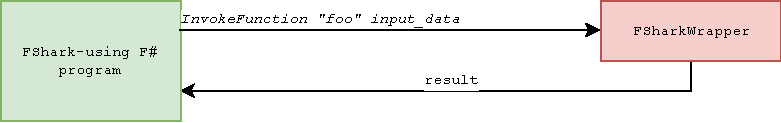
\includegraphics{chapters/figs/csharp/pipeline_step_3.pdf}
  \caption{The \fshark{} compilation pipeline}
  \label{fig:fsharkcompilerpipeline}
\end{figure}


When calling \texttt{CompileAndLoad}, the supplied \fshark{} source files are
concatenated into one long source file, and written to a temporary location.
An FSharpChecker is then initialized, so we can parse and type check the
concatenated source code. The FSharpChecker is a class exported by the FSharp
Compiler Services, and is a class that lets developers use part of the F\#
compilation pipeline at runtime.

We supply the FSharpChecker with the path to our precompiled \fshark{}Prelude
assembly, and then call its \texttt{ParseAndCheckProject} method on to receive
an assembly value, which contains the complete Typed Abstract Syntax Tree of our
\fshark{} program, in the form of an \texttt{FSharpImplementationFileDeclaration}.

If the \fshark{} developer followed the guidelines to write a well-formed FShark
module, the main declaration of the program, the
\texttt{FSharpImplementationFileDeclaration}, should contain a single
\texttt{FSharpEntity}, which in turn contains all the remaining declarations in
the program.

\subsubsection*{The declaration types within F\#'s Typed AST}
The \texttt{FSharpImplementationFileDeclaration} type has three union cases.
\begin{description}
\item[\texttt{InitAction of FSharpExpr}] \hfill\\
  \texttt{InitAction}s are \fsharpexpr{}s that are executed at the
  initialization of the containing entity. These are not supported in \fshark{}.

\item[\texttt{Entity of FSharpEntity * FSharpImplementationFileDeclaration list}]\hfill\\
  An \texttt{Entity} is the declaration of a type or a module. In the case of
  \fshark{}, three different kinds of entities are supported:
  \begin{description}
  \item[FSharpRecords] are standard record types, and can be translated to
    Futhark records with ease.
    This entity has an empty \texttt{FSharpImplementationFileDeclaration list}.
  \item[FSharpAbbreviations] are type abbreviations, and are easily translated
    into Futhark type aliases.
    This entity has an empty \texttt{FSharpImplementationFileDeclaration list}.
  \item[FSharpModules] are named modules which contains subdeclarations.
    In this case, we retrieve the subdeclarations from the \texttt{FSharpImplementationFileDeclaration list}.
    The \fshark{} compiler supports building FShark modules, but current
    limitations demands that modules are flattened when compiled to Futhark.
    This also means that function name prefixes in function calls are stripped
    when compiled to Futhark.
  \end{description}
\item[\texttt{MemberOrFunctionOrValue of \\ FSharpMemberOrFunctionOrValue *
    FSharpMemberOrFunctionOrValue list list * FSharpExpr}]\hfill\\
  F\# doesn't differ between functions and values, which means that a function
  is merely a value with arguments.
  A pattern matched \texttt{MemberOrFunctionOrValue} value has the form
  \texttt{MemberOrFunctionOrValue (v, args, exp)}, where \texttt{v} contains the
  name and the type of the variable.
  If the \texttt{args} list is empty, \texttt{v} is simply a variable. If not,
  \texttt{v} is a function. \texttt{exp} contains the \fsharpexpr{} that
  \texttt{v} is bound to. An \fsharpexpr{} can be anything from a numeric
  constant to a very long function body.
\end{description}

In figure \ref{fig:validfsharkprogram} we see a small but valid \fshark{} program. It
reads like a regular F\# program, but contains the three vital parts that makes
it usable as an \fshark{} program.

\begin{figure}[h]
  \centering
  \begin{minted}[xleftmargin=5pt,linenos]{fsharp}
    module ExampleModule
    open FSharkPrelude

    module SomeValues =
      let Four : int = 4

      let SomePlus (x : int) (y : int) : int = x + y

    [<FSharkEntry>]
    let TimesTwo (x : int) : int =
      SomeValues.SomePlus x x
  
    [<FSharkEntry>]
    let MapPlusTwo (xs : int array) : int array =
      Map ((+)2) xs

    let PlusSeven (x : int) : int =
      SomeValues.SomePlus x 7
  \end{minted}
  \caption{A valid \fshark{} program}
  \label{fig:validfsharkprogram}
\end{figure}

\begin{itemize}
\item The module declaration on the first line declares that the following code
  is inside a module. In this case, we are declaring the module
  \texttt{ExampleModule}, although we could use any valid F\# module name.
  As shown in figure \ref{fig:validfsharkprogramresult}, the top module
  declaration falls away during compilation, so only the top module contents are
  left.

\item This \texttt{open} statement ensures that the F\# Compiler Services has
  access to the \fshark{}Prelude during the compilation. It is possible to write an
  \fshark{} program which doesn't use the FSharkPrelude, but this removes access to
  the SOACs that we use to write our data parallel programs.

\item The \texttt{[<\fshark{}Entry>]} attributed function \texttt{TimesTwo} ensures
  that the resulting Futhark library from the \fshark{} compiler has at least one
  entry point function.
  Without any entry point functions, we won't have any functions in the final
  compiled \fshark{} program.
\end{itemize}

\begin{figure}
  \centering
\begin{lstlisting}[language=Futhark]
    let Four : i32 = 4i32
    let SomePlus (x : i32) (y : i32) : i32 =
      ((x i32.+ y))
    entry TimesTwo (x : i32) : i32 =
      unsafe SomePlus(x) (x)
    entry MapPlusTwo (xs : []i32) : []i32 =
      unsafe map (let x = 2i32 in
                  (\(y : i32) -> ((x i32.+ y)))) (xs)
    let PlusSeven (x : i32) : i32 =
      SomePlus(x) (7i32)
      \end{lstlisting}
  \caption{A valid \fshark{} program, compiled to Futhark}
  \label{fig:validfsharkprogramresult}
\end{figure}

In figure \ref{fig:validfsharkprogramresult} we see the resulting Futhark program.
For now, we will ignore the transformations that have happened, except for two
things: The \texttt{Map} function (called from \fshark{}Prelude) has been rewritten
as the plain Futhark SOAC \texttt{map} in lowercase, and the module SomeValues has been
flattened (see sec \ref{futurework:modules} for future plans.)

This Futhark program is then stored in a temporary location in the user's file
system, and compiled into as a library, using Futhark's C\# compiler, either
with or without OpenCL support. Finally after this compilation, we can invoke
the resulting .dll file from within the \fshark{}-using F\# program.

\subsection*{Building \fshark{} from the Typed AST}
\label{sec:fsharkcompilerrules}
Only the supported FSharpExpr's has been listed here, but the full range of
FSharpExpr's are available on \cite{typedtree}.

\subsection*{FSharp-to-\fshark{}IL rules}
INTRODUCTION HERE

For these translations, we will disregard that all \fsharpexpr{}s are union
cases of the F\# data type \texttt{BasicPatterns}.


\begin{figure}
  \begin{framed}
    
  \centering
\begin{tabular}{@{}l c l}% to \linewidth {l c X}
  $\evals{Entity(\lit{IsFSharpRecord}, [(field_0 : \tau_0), \ldots, (field_n : \tau_n)])}$ & & \\
  $= \lit{FSharkRecord([}(field_0 : \evals{\tau_0}), \ldots, (field_n : \evals{\tau_n})\lit{])}$ & & \\
  ~ \\
\end{tabular}
\begin{tabular}{@{}l c l}% to \linewidth {l c X}
  $\evals{Entity(\lit{IsFSharpTypeAbbreviation}, alias, \tau)}$ & & \\
  $= \lit{FSharkTypeAlias(} alias, \evals{\tau}\lit{)}$ & & \\
  ~ \\
\end{tabular}
\begin{tabular}{@{}l c l}% to \linewidth {l c X}
  $\evals{Entity(\lit{IsFSharpModule}, [decl_0,\ldots,decl_n])}$ & & \\
  $= [\evals{decl_0},\ldots,\evals{decl_n}]$ & & \\
  ~ \\
\end{tabular}
\begin{tabular}{@{}l c l}% to \linewidth {l c X}
  $\evals{MemberOrFunctionOrValue((name, \tau^{*}, IsEntryFunction), [(arg_0 : \tau_0), \ldots, (arg_n : \tau_n)], e)}$ & & \\
  $= FSharkVal(IsEntryFunction, \lit{FSharkFunction}([\evals{\tau_0}, \ldots, \evals{\tau_n}], \evals{\tau^{*}}),name, [arg_0,..,arg_n],\evals{e})$ & & \\
  ~ \\
\end{tabular}
\caption{Rules for translating FSharp declarations to FShark
    declarations}
  \end{framed}

\end{figure}


\begin{figure}
  \centering
\begin{tabular}{@{}l c l}% to \linewidth {l c X}
  $\evals{System.Int8}$ & $=$ & $\lit{FInt8} $ \\ 
  $\evals{System.Int16}$ & $=$ & $\lit{FInt16}$
  \\
  $\evals{System.Int32}$ & $=$ & $\lit{FInt32} $ \\ 
  $\evals{System.Int64}$ & $=$ & $\lit{FInt64} $
  \\
  $\evals{System.UInt8}$ & $=$ & $\lit{FUInt8} $ \\ 
  $\evals{System.UInt16}$ & $=$ & $\lit{FUInt16} $ 
  \\
  $\evals{System.UInt32}$ & $=$ & $\lit{FUInt32} $ \\ 
  $\evals{System.UInt64}$ & $=$ & $\lit{FUInt64} $ 
  \\
  $\evals{System.Single}$ & $=$ & $\lit{FSingle} $ \\ 
  $\evals{System.Double}$ & $=$ & $\lit{FDouble} $ 
  \\
  $\evals{System.Boolean}$ & $=$ & $\lit{Bool} $ \\ 
  $\evals{System.Array~\tau}$ & $=$ & $\lit{\fshark{}Array }\evals{\tau}$
  \\
  $\evals{System.Tuple~(\tau_0 \times \ldots \times \tau_n)}$ & $=$ & $\lit{\fshark{}Tuple}~(\evals{\tau_0}~\times~\ldots~\times~\evals{\tau_n)}$ \\ ~ \\
\end{tabular}

INSERT NOTE ON RULE FOR TUPLE ('a [] * long [])

\caption{Rules for translating .NET types to FSharkIL types}
\end{figure}

\begin{figure}
  \centering
\begin{tabular}{@{}l c l}% to \linewidth {l c X}
  $\evals{\lit{FInt8}}$ & $=$ & $\lit{i8} $ \\ 
  $\evals{\lit{FInt16}}$ & $=$ & $\lit{i16}$
  \\              
  $\evals{\lit{FInt32}}$ & $=$ & $\lit{i32} $ \\ 
  $\evals{\lit{FInt64}}$ & $=$ & $\lit{i64} $
  \\
  $\evals{\lit{FUInt8}}$ & $=$ & $\lit{u8} $ \\ 
  $\evals{\lit{FUInt16}}$ & $=$ & $\lit{u16} $ 
  \\               
  $\evals{\lit{FUInt32}}$ & $=$ & $\lit{u32} $ \\ 
  $\evals{\lit{FUInt64}}$ & $=$ & $\lit{u64} $ 
  \\
  $\evals{\lit{FSingle}}$ & $=$ & $\lit{f32} $ \\ 
  $\evals{\lit{FDouble}}$ & $=$ & $\lit{f64} $ \\
  $\evals{\lit{Bool}}$ & $=$ & $\lit{bool} $ \\ 
  $\evals{\lit{FSharkArray}~\tau}$ & $=$ & $\lit{[]}\evals{\tau}$
  \\
  $\evals{\lit{\fshark{}Tuple}~({\tau_0}~\times~\ldots~\times~{\tau_n})}$ & $=$ & $(\evals{\tau_0},\ldots,\evals{\tau_n})$ \\ ~ \\
\end{tabular}
\caption{\texttt{\fshark{}IL} types to Futhark types}
\end{figure}

\begin{figure}
  \centering
  \begin{tabular}{@{}l c l}% to \linewidth {l c X}
  $\evals{Const(obj, \tau)}$ & $=$ & $\lit{Const(}obj, \evals{\tau} \lit{)}$ \\
  $\evals{Value(v)}$ & $=$ & $\lit{Var(}v{)}$ \\
  $\evals{AddressOf(v)}$ & $=$ & $\evals{v}$ \\
  $\evals{NewTuple(\_, [e_0,...,e_1])}$ & $=$ & $\lit{Tuple([}\evals{e_0},\ldots, \evals{e_n}\lit{])}$ \\
  $\evals{NewRecord((v_0 : \tau_0 * \ldots * v_n : \tau_n), [e_0,...,e_1])}$ & $=$ & $\lit{Record([}(v_0,\evals{e_0}),\ldots,(v_n,\evals{e_n})\lit{])}$ \\
  $\evals{NewArray(\tau, [e_0,...,e_1])}$ & $=$ & $\lit{List(}\evals{\tau},\lit{[}\evals{e_0},\ldots, \evals{e_n}\lit{]}\lit{)}$ \\
  $\evals{TupleGet(\_, i, e)}$ & $=$ & $\lit{TupleGet(}\evals{e}, i{)}$ \\
  $\evals{FSharpFieldGet(e, \_, field)}$ & $=$ & $\lit{RecordGet(}field, \evals{e}{)}$ \\
    $\evals{Call(\_, \lit{GetArray}, \_, nil, [e_0, e_1])}$ & $=$ & $\lit{ArrayIndex(}\evals{e_0},\evals{e_1}]\lit{)}$ \\
    $\evals{Call(\_, name, \_, nil, [e_0, \ldots, e_n])}$ & $=$ & $\lit{Call(}name, [\evals{e_0},\ldots,\evals{e_n}]\lit{)}$ \\
    $\evals{Call(\_, name, \_, \tau, [e_0, \ldots, e_n])}$ & $=$ & $\lit{TypedCall(}\evals{\tau},name, [\evals{e_0}, \ldots, \evals{e_n}]\lit{)}$ \\
    $\evals{Call(\_, infixOp, \_, \tau, [e_0, e_1])}$ & $=$ & $\lit{InfixOp(}infixOp, \evals{\tau}, \evals{e_0}, \evals{e_1}\lit{)}$ \\
    $\evals{Call(\_, unaryOp, \_, \tau, [e_0])}$ & $=$ & $\lit{UnaryOp(}unaryOp, \evals{\tau}, \evals{e_0}\lit{)}$ \\
  $\evals{Let(v, e_0, e_1)}$ & $=$ & $\lit{LetIn(}v, \evals{e_0}, \evals{e_1}\lit{)}$ \\
  $\evals{IfThenElse(e_0, e_1, e_2)}$ & $=$ & $\lit{If(}\evals{e_0}, \evals{e_1}, \evals{e_2}\lit{)}$ \\
  $\evals{Lambda((v : \tau), e)}$ & $=$ & $\lit{Lambda(}v, \evals{\tau}, \evals{e} \lit{)}$ \\
  $\evals{Application(func, \_, [e_0, \ldots, e_n])}$ & $=$ & $\lit{Application(}\evals{func}, \lit{[}\evals{e_0},\ldots, \evals{e_n}\lit{])}$ \\
  $\evals{TypeLambda(e)}$ & $=$ & $\evals{e}$ \\
  $\evals{DecisionTree(\_, \_)}$ & $=$ & $\lit{Pass}$ \\
  $\evals{DecisionTreeSuccess(\_, \_)}$ & $=$ & $\lit{Pass}$ \\ ~ \\
\end{tabular}
\caption{Translation rules for FSharp expressions to FSharkIL expressions}
\end{figure}

  
\begin{figure}
  \centering
  \begin{tabular}{@{}l c l}% to \linewidth {l c X}
  $\evals{Const(obj, \tau )}$ & $=$ & $obj\evals{\tau}$ \\
  $\evals{Var(v)}$ & $=$ & $v$\\
  $\evals{Tuple([e_0,\ldots, e_n])}$ & $=$ & $(\evals{e_0},\ldots, \evals{e_n})$\\
  $\evals{Record([(v_0, e_0),\ldots,(v_n,e_n)])}$ & $=$ & $\{v_0=\evals{e_0},~\ldots,~v_n=\evals{e_n}\}$ \\
  $\evals{List(}\evals{\tau},\lit{[}\evals{e_0},\ldots, \evals{e_n}\lit{]}\lit{)}$ & $=$ & $[\evals{e_0},~\ldots,~\evals{e_n}]$\\
  $\evals{TupleGet(}\evals{e}, i{)}$ & $=$ & $\evals{e}.i$ \\
  $\evals{RecordGet(field, e)}$ & $=$ & $\evals{e}.field$ \\
  $\evals{ArrayIndex(e_{arr},[e_0, \ldots, e_n])}$ & $=$ & $\evals{e_{arr}}\lit{[}\evals{e_0},\ldots,\evals{e_n}\lit{]}$ \\
    
  $\evals{Call(name, [e_0,\ldots,e_n]\lit{)}}$ & $=$ & $name~(\evals{e_0})~\ldots~(\evals{e_n})$ \\
  $\evals{TypedCall(}\evals{\tau},name, [\evals{e_0}, \ldots, \evals{e_n}]\lit{)}$ & $=$ & $\evals{\tau}.name~(\evals{e_0})~\ldots~(\evals{e_n})$ \\
  $\evals{InfixOp(}infixOp, \evals{\tau}, \evals{e_0}, \evals{e_1}\lit{)}$ & $=$ & $(\evals{e_0})~\evals{\tau}.infixOp~(\evals{e_1})$ \\
  $\evals{UnaryOp(}unaryOp, \evals{\tau}, \evals{e_0}\lit{)}$ & $=$ & $\evals{\tau}.unaryOp~(\evals{e_0})$ \\

  $\evals{LetIn(}v, \evals{e_0}, \evals{e_1}\lit{)}$ & $=$ & $\mathtt{let}~v~=~\evals{e_0}~\mathtt{in}~\evals{e_1}$ \\

  $\evals{If(}\evals{e_0}, \evals{e_1}, \evals{e_2}\lit{)}$ & $=$ & $\mathtt{if}~\evals{e_0}~\mathtt{then}~\evals{e_1}~\mathtt{else}~\evals{e_2}$ \\

  $\evals{Lambda(v, \evals{\tau}, \evals{e} \lit{)}}$ & $=$ & $\mathtt{\backslash}(v : \evals{\tau})~\mathtt{->}~\evals{e}$ \\
  $\evals{Application(\evals{func}, \lit{[}\evals{e_0},\ldots, \evals{e_n}\lit{])}}$ & $=$ & $(\evals{func})~(\evals{e_0})~\ldots~(\evals{e_n})$ \\
  $\evals{Pass}$ & $=$ & $\epsilon$ $$ \\
\end{tabular}
\caption{\texttt{FSharkIL} expressions to Futhark}
\end{figure}

\section{Design choices in writing the FShark Compiler}
% should I write parser manually or just use FSharp library
% this meant a design process where I disected F# programs using Riders debugger

% biggest hurdle for compiler: updated Futhark lang specifications: 

% what could be expanded?
% maybe make a loop function that imitates the futhark loop construct

%%% Local Variables:
%%% mode: latex
%%% TeX-master: "../thesis"
%%% End: